% 
%  chapter4.tex
%  ISELthesis
%  
%  Created by Matilde Pós-de-Mina Pato on 2012/10/09.
%
\chapter{Implementation}
\label{cha:impl}

This chapter describes how the architecture and resolution cascade introduced in
Chapter~\ref{ch:proposed_solution} are realised in code. It follows the same two-part structure
as the contribution itself: the Function Registry and the deployment-time resolution mechanism
shared by both cloud providers, and the AWS Lambda support added to QuickFaaS that the
AWS-side resolver and deployer depend on.

The chapter is organised in three sections. Section~\ref{sec:function-registry} presents the
Function Registry itself: its file format, how entries are created and kept up to date, and the
internal behaviour of the two provider resolvers that consult it at deployment time. The
following section, AWS Lambda Support in QuickFaaS, traces the concrete deployment steps that
Level~3 of the cascade triggers on AWS --- work that has no equivalent on the GCP path.
Section~\ref{sec:runtime-invocation} closes the chapter by following a resolved internal call
through to its actual invocation once the workflow has been deployed.

\section{Function Registry}
\label{sec:function-registry}

This work introduces a \textit{Function Registry} to decouple workflow definitions from concrete function endpoints, reducing manual coordination between function deployments and workflow orchestration.

Figure~\ref{fig:omniflow-integration-classes} details the classes that realise the unification inside OmniFlow. Function deployment is abstracted behind the \texttt{InternalFunctionDeployer} interface, following the strategy pattern, with three implementations: \texttt{Noop\allowbreak Internal\allowbreak Function\allowbreak Deployer} (the safe default, which raises if invoked), \texttt{QuickFaasDeployer} (GCP), and \texttt{AwsLambdaDeployer} (AWS, added in this work). Each provider deployer (\texttt{GoogleCloudDeployer}, \texttt{AmazonCloudDeployer}) owns a provider-specific resolver, and both resolvers share two collaborators: the \texttt{FunctionRegistryStore}, which persists bindings as \texttt{FunctionInvocationMetadata} (\texttt{serviceName} plus \texttt{url}, where \texttt{url} is an HTTPS endpoint on GCP and a Lambda ARN on AWS), and the deployer strategy. The \texttt{Function\allowbreak Registry\allowbreak Bootstrapper} populates a missing registry by discovery. This structure keeps the two providers symmetric and makes the deployer a clean extension point: supporting a further platform means adding one resolver and one \texttt{InternalFunctionDeployer}, without touching the existing ones.
\begin{figure}[htbp]
  \centering
  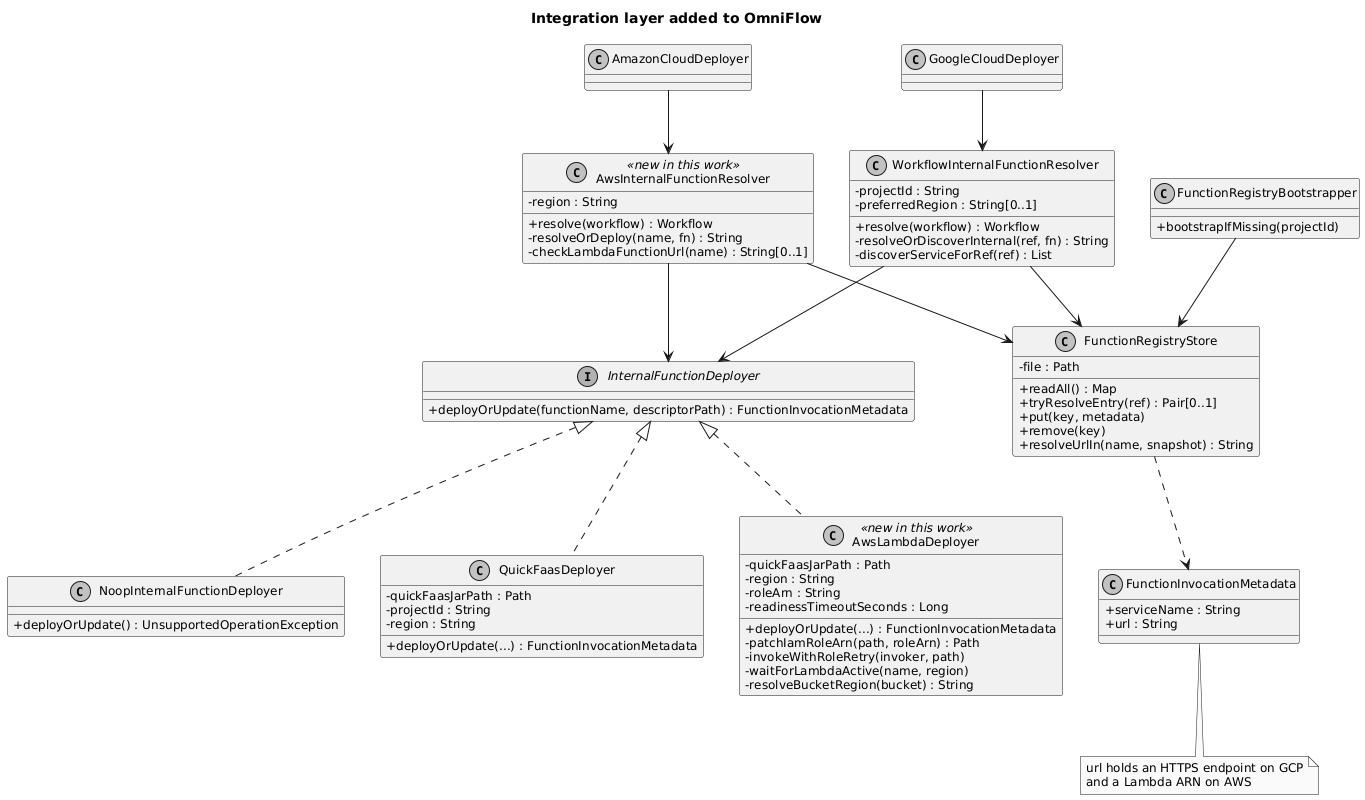
\includegraphics[width=\textwidth]{images/implementation/omniflow-integration-classes.png}
  \caption{Class model of the integration layer added to OmniFlow.}
  \label{fig:omniflow-integration-classes}
\end{figure}


\subsection{Motivation}
In the original OmniFlow usage model, a \texttt{call} step requires concrete endpoint information (namely \texttt{host} and \texttt{path}). This makes workflows brittle: if a function is redeployed and its endpoint changes, the workflow definition must also be updated. The Function Registry addresses this problem: workflows reference internal functions through stable logical identifiers instead of concrete endpoints. The actual endpoint is only bound to that identifier at deployment time. Beyond endpoint indirection, the registry also serves as the persistence layer for the
automatic function resolution mechanism described below: entries are created and refreshed
automatically as functions are discovered on the target provider or deployed through QuickFaaS.



\subsection{Concept and Conventions}
Each internal function is identified by a stable logical identifier, referred to as
\texttt{functionRef} (e.g., \texttt{"fraud-check"}). Instead of embedding the real endpoint
in the workflow definition, an internal call declares the function through a dedicated DSL
construct, \texttt{internalFunction(name, deploymentDescriptorPath)}, added to the
\texttt{call} step in this work. The two construction paths are mutually exclusive and
enforced at build time:

\begin{itemize}
    \item \textbf{External calls} provide literal \texttt{host} and \texttt{path} values,
    exactly as in the original OmniFlow design, and bypass the registry entirely.
    \item \textbf{Internal calls} provide \texttt{internalFunction(...)} and \emph{must not}
    set \texttt{host} or \texttt{path}: both fields are filled in automatically at deployment
    time from the registry. The optional second argument points to a QuickFaaS deployment
    descriptor, used only when the function cannot be resolved or discovered (see below).
\end{itemize}

For example, an internal function call is declared as:

\begin{lstlisting}[language=Kotlin,caption={Internal call declared with \texttt{internalFunction}},label={lst:internal-call-registry}]
call {
    method(GET)
    internalFunction(
        "fraud-check",
        deploymentDescriptorPath = "./functions/fraud-check/func-deployment.json"
    )
    result("fraudResult")
}
\end{lstlisting}

External calls are unaffected by this mechanism: they continue using literal \texttt{host} and \texttt{path} values and bypass the registry resolution.

\subsection{Registry File Format}
The registry is stored as a JSON file, containing only non-secret invocation metadata. It maps each \texttt{functionRef} to the concrete values required to invoke the function (serviceName and url, where url is an HTTPS endpoint on GCP and a Lambda ARN on AWS). The registry also stores an \texttt{updatedAt} timestamp for traceability.

\begin{lstlisting}[language=json,caption={Function registry structure},label={lst:function-registry}]
{
  "updatedAt": "2026-02-15T00:00:00Z",
  "functions": {
    "fraud-check": {
      "serviceName": "fraud-check",
      "url": "https://fraud-check-abc123-ew.a.run.app"
    },
    "europe-west1/risk-score": {
      "serviceName": "risk-score",
      "url": "https://risk-score-def456-ew.a.run.app"
    },
    "hello-lambda-fn": {
      "serviceName": "hello-lambda-fn",
      "url": "arn:aws:lambda:eu-west-1:123456789012:function:hello-lambda-fn"
    }
  }
}
\end{lstlisting}

\subsection{Creation, Bootstrap and Updates}
The registry management layer provides the following behavior:

\begin{itemize}
    \item \textbf{Bootstrap by discovery:} if the registry file does not exist, it is created
    automatically by listing the functions already deployed on the target provider --- Cloud Run
    services on GCP, Lambda functions on AWS --- and writing one entry per discovered function; on
    AWS this scans every region enabled for the account and, mirroring the GCP catalog, promotes a
    function name seen in more than one region from a bare key to a \texttt{"region/name"} key for
    each occurrence.
    \item \textbf{Automatic registration:} when an internal function is not present in the
    registry but is found on the target provider (Cloud Run service on GCP, Lambda function
    on AWS), a new entry is written immediately with the discovered metadata.
    \item \textbf{Post-deployment updates:} after a successful QuickFaaS deployment, the
    resulting invocation metadata is written to the registry, so subsequent deployments
    resolve the function without redeploying it.
    \item \textbf{Drift handling:} on every registry hit, the stored endpoint is validated
    against the live resource (Cloud Run service on GCP, Lambda function on AWS); if it
    changed, the entry is refreshed, and if the resource no longer exists, the stale entry is
    removed and deployment fails with an explicit diagnostic.
\end{itemize}

Every write refreshes the top-level \texttt{updatedAt} timestamp.

\subsection{Deployment-Time Endpoint Resolution}
\label{subsec:endpoint-resolution}
The registry is consumed at deployment time by an endpoint resolution step. Before rendering the provider-specific workflow artifact (e.g., Google Workflows YAML), OmniFlow inspects each \texttt{CallContext}:

\begin{enumerate}
    \item OmniFlow traverses the workflow tree (including nested branches, iterations and
    parallel blocks) and intercepts every \texttt{CallContext} carrying an
    \texttt{internalFunction} declaration; external calls are left untouched.
    \item The registry is consulted for the \texttt{functionRef} (exact match first, then
    suffix match on \texttt{"region/functionRef"}). On a hit, the stored URL is used --- on
    GCP, after validating it against the live Cloud Run service.
    \item On a registry miss, the target provider is queried directly (Cloud Run service
    lookup across regions on GCP; on AWS, a \texttt{GetFunction} lookup across every region
    enabled for the account, or a single call when the fully-qualified form is used). If the function
    exists, its metadata is registered and used --- no deployment is triggered.
    \item Only if the function is absent from both the registry and the provider, and a
    \texttt{deploymentDescriptorPath} was declared, is QuickFaaS invoked to deploy the
    function; the returned metadata is registered and used. Otherwise, deployment fails
    fast with a diagnostic identifying the unresolved function.
\end{enumerate}

The resolved URL is finally split into \texttt{host} and \texttt{path} (on AWS, into a
\texttt{lambda://<arn>} reference consumed by the renderer) and injected into the call step
before the provider-specific workflow artifact is rendered.

\subsection{Registry Store and Resolver Internals}
\label{subsec:store-internals}

The registry file is manipulated exclusively through \texttt{FunctionRegistryStore}, which
exposes a small, deliberately narrow interface: \texttt{readAll()} parses the whole file into an
ordered map of \texttt{functionRef} to \texttt{FunctionInvocationMetadata}; \texttt{tryResolveEntry()}
re-reads the file via \texttt{readAll()} and delegates the two-step lookup (exact match on
\texttt{functionRef}, then suffix match on \texttt{"region/functionRef"}, raising if the suffix
match is ambiguous) entirely to its pure counterpart, \texttt{tryResolveEntryIn()}, which performs
that lookup against an already-loaded map with no I/O of its own --- the same split
\texttt{resolveUrl()}/\texttt{resolveUrlIn()} already had; \texttt{put()} inserts or refreshes one entry; and
\texttt{remove()} deletes a stale entry. Every mutating operation rewrites the top-level
\texttt{updatedAt} timestamp. The store itself keeps no in-memory state between calls, so
\texttt{readAll()}/\texttt{tryResolveEntry()} re-read and re-parse the file on every call; the
performance consequences of this choice, and the single-read mitigation built on
\texttt{tryResolveEntryIn()}, are analysed in Chapter~\ref{cha:evaluation}.

The two provider resolvers sit on top of this store and are now symmetric in shape, differing only
in the provider-discovery calls that reflect the two clouds' invocation models.
\texttt{Workflow\allowbreak Internal\allowbreak Function\allowbreak Resolver} (GCP) treats a registry hit as provisional: it
validates the stored URL against the live Cloud Run service and, if the URL has drifted, refreshes
the entry; if the service has disappeared, it attempts rediscovery across the project's regions
and, failing that, removes the stale entry and aborts. It also short-circuits validation for
first-generation Cloud Functions (identified by a \texttt{cloudfunctions.net} URL), which are not
Cloud Run services. When a function is absent from the registry, it is looked up across regions,
and a match in more than one region is reported as ambiguous.
\texttt{Aws\allowbreak Internal\allowbreak Function\allowbreak Resolver} follows the same shape: it treats a registry hit
as provisional, resolving the region to validate from the stored ARN and consulting the Lambda API
through a \texttt{Lambda\allowbreak Function\allowbreak Inspector} seam; a drifted ARN refreshes the entry, and a
permissions failure aborts rather than being mistaken for an absence. What used to be the one
AWS-only shortcut --- a Lambda name is unique within its region, so a hit's validation was a single
\texttt{GetFunction} call with no cross-region fallback --- no longer holds: on a \texttt{NotFound}
result (or an unparseable stored ARN), the resolver now mirrors the GCP path and attempts
rediscovery, searching every region enabled for the account before removing the stale entry and
aborting. Region discovery is itself provider-specific: GCP already exposed a project-scoped
locations API, whereas AWS has no equivalent for Lambda, so a dedicated
\texttt{Ec2Aws\allowbreak Regions\allowbreak Lister}, backed by the EC2 \texttt{DescribeRegions} call, was added to
play that role; an optional preferred region, when supplied, is tried first in both the
rediscovery and the miss-path scan described next. On a registry miss, the AWS resolver now performs
the same style of scan as GCP: it searches every enabled region for a function-name match,
disambiguating a name found in more than one region, unless the caller supplies the
fully-qualified \texttt{"<region>/<functionRef>"} form, which resolves a single region directly. A
region reporting \texttt{ResourceNotFoundException} and one reporting a permissions failure are
both simply excluded from the candidate set while the scan runs, but the two are told apart at the
end, exactly as on the GCP path: if the function is found in no region and at least one of the
scanned regions was inaccessible, the resolver raises a diagnostic naming those regions instead of
concluding the function is absent everywhere; the absence conclusion is only drawn when every
scanned region reported a clean \texttt{NotFound}. This closes the asymmetry the miss path used to
have, where a single \texttt{GetFunction} call collapsed a genuine absence and a permissions
failure into the same outcome (see \S\ref{subsec:validation-error-semantics}). What now
distinguishes the two resolvers is only the underlying provider API each one calls --- the Cloud
Run Locations API versus EC2 \texttt{DescribeRegions} for region discovery, a Cloud Run lookup
versus \texttt{GetFunction} for the per-region check --- and the GCP-only short-circuit for
first-generation Cloud Functions noted above, which has no AWS counterpart. In both resolvers, a hit or a
successful discovery writes the metadata back through \texttt{put()} before the endpoint is
injected into the call, so the registry converges toward a complete set of bindings as workflows
are deployed.

To keep resolution cheap when a workflow contains many internal calls, both provider resolvers
read the registry once into a snapshot at the start of \texttt{resolve()} and resolve every call
against that in-memory map, keeping it in sync with every subsequent \texttt{put()}/\texttt{remove()}
so that two calls to the same function within one workflow still observe each other's writes,
rather than re-reading the file per call. This is the optimisation quantified in
Chapter~\ref{cha:evaluation} (Section~\ref{sec:eval-real-resolvers}), first demonstrated on a
now-removed reference resolver (\S\ref{subsec:store-internals}) and since folded into
\texttt{Aws\allowbreak Internal\allowbreak Function\allowbreak Resolver} and
\texttt{Workflow\allowbreak Internal\allowbreak Function\allowbreak Resolver} themselves.

\subsection{Resolution Cascade Sequences}
\label{subsec:cascade-sequences}

The description of the two resolvers above is expanded into six sequence diagrams, one per
cascade level and provider, making explicit the messages exchanged with the registry and with
each provider's inspection API; to keep this chapter's flow uninterrupted, the diagrams themselves
are collected in Appendix~\ref{app:cascade-sequences} rather than placed inline.

Figure~\ref{fig:resolution-cascade-level1} (Appendix~\ref{app:cascade-sequences}) details Level~1
on each provider: a registry hit is validated against the live resource before being trusted. The
two panels now show matching behaviour on a \texttt{NotFound} result --- both the GCP path (a) and
the AWS path (b) attempt rediscovery across every region before removing the stale entry and
aborting, now that AWS validation is no longer pinned to the region recorded in the stored ARN.

Figure~\ref{fig:resolution-cascade-level2} (Appendix~\ref{app:cascade-sequences}) details Level~2,
reached on a registry miss. Both resolvers now search across every region --- the GCP path (a)
across the project's regions, the AWS path (b) across every region enabled for the account,
discovered via EC2 \texttt{DescribeRegions} --- or a single region when the fully-qualified
\texttt{"region/functionRef"} form is used, reporting more than one match as ambiguous. On both
paths, a per-region permissions failure is not distinguished from a genuine absence in that region
while at least one other region remains reachable, but if no match is found anywhere and at least
one region was inaccessible, the resolver reports the inaccessible regions explicitly rather than
treating the miss as a plain absence (\S\ref{subsec:validation-error-semantics}).

Figure~\ref{fig:resolution-cascade-level3} (Appendix~\ref{app:cascade-sequences}) details Level~3,
reached only when a \texttt{deploymentDescriptorPath} was supplied and the function was found on
neither the registry nor the provider. Both panels stay at the cascade's conceptual level; the
full operational breakdown of the AWS branch --- the IAM role, the region derived from the S3
bucket, subprocess retries, and \texttt{GetFunction} polling --- is traced separately for the
worst-case path in Figure~\ref{fig:aws-deploy-sequence}, introduced in the AWS Lambda Support
section that follows.

\subsection{Validation and Error Semantics}
\label{subsec:validation-error-semantics}
Several correctness constraints are enforced to avoid silent misconfiguration:

\paragraph{Unresolvable function.}
If a function is absent from the registry and from the target provider, and no deployment
descriptor was provided, deployment fails fast with a message identifying the function and
the corrective actions (deploy it first, or provide \texttt{deploymentDescriptorPath}).

\paragraph{Ambiguous references.}
If a suffix match yields multiple regional entries in the registry, or a function name
exists in multiple regions on the provider, deployment fails with a message instructing the
developer to disambiguate using the fully-qualified form
\texttt{internalFunction("<region>/<functionRef>")}. Unlike an unresolvable function, this
failure is not rescued by supplying a \texttt{deploymentDescriptorPath}: ambiguity is a
data-consistency problem, not an absence one, so QuickFaaS is never invoked to paper over it.

\paragraph{Stale registry entries.}
If a registry entry points to a resource that no longer exists --- a Cloud Run service on GCP, or
a Lambda on AWS, for which rediscovery across every region also fails --- the stale entry is
removed and deployment aborts with an explicit diagnostic, preventing the workflow from being
deployed against a dead endpoint.

\paragraph{Insufficient permissions.}
If the live lookup used to validate a registry hit is refused (an authorization failure rather
than an absence), deployment aborts immediately with a diagnostic naming the function; on GCP no
rediscovery is attempted, since a permissions failure gives no information about whether the
service still exists. The same rule now applies on AWS, where a refused \texttt{GetFunction} is
likewise distinguished from a genuine absence. The distinction is drawn more coarsely on the
miss-path region scan, on both providers: while the scan is running, a region where the lookup is
refused is simply excluded from the candidate set, the same as a region where the function is
absent, so a permissions gap in one region does not by itself stop a match found elsewhere; but if
the scan ends with no match anywhere and at least one region could not be checked, it surfaces a
diagnostic naming the inaccessible regions instead of silently concluding the function is absent
everywhere (see \S\ref{subsec:store-internals}).

\subsection{Registry Location}
The registry file is stored in a writable location at runtime (e.g., the working directory or a configurable path provided to the deployer). This avoids attempting to write into packaged resources (which are typically read-only in production).

\subsection{Evolution of the Registry Design}
\label{subsec:registry-evolution}

The registry did not arrive at its current form in a single step; the source tree still exposes
the intermediate stages, which makes the design decisions worth recounting. Five threads describe
how it evolved.

\paragraph{From literal endpoints to logical indirection.}
The starting point was the plain OmniFlow \texttt{call} step, which embeds a concrete
\texttt{host}/\texttt{path}. This couples the workflow definition to a specific deployed instance
of a function, so any redeployment that changes the endpoint forces an edit to the workflow. The
first design move was therefore to introduce a level of indirection: the workflow names a function
through a stable \texttt{functionRef}, and the concrete endpoint is bound from the registry at
deployment time. The registry exists precisely to hold that binding.

\paragraph{From a two-key model to a metadata record.}
An early registry design represented each function by two synthetic keys,
\texttt{"<functionRef>.host"} and \texttt{"<functionRef>.path"}, produced by
\texttt{FunctionEndpointKeys} and consumed by \texttt{Workflow\allowbreak Internal\allowbreak Call\allowbreak Endpoint\allowbreak Resolver}. This
mirrored the \texttt{host}/\texttt{path} split of the \texttt{call} step but proved awkward: it
stored two loosely related string fragments per function and pushed the reconstruction of a full
endpoint onto the resolver. It was superseded by a single structured record per function,
\texttt{FunctionInvocationMetadata} (a \texttt{serviceName} plus a \texttt{url}), which the two
production resolvers consume. \texttt{FunctionEndpointKeys} was simply deleted once nothing
referenced it, but \texttt{Workflow\allowbreak Internal\allowbreak Call\allowbreak Endpoint\allowbreak Resolver} held something worth
keeping first: the single-read registry optimization it demonstrated (Section~\ref{sec:eval-resolution})
was propagated into \texttt{Aws\allowbreak Internal\allowbreak Function\allowbreak Resolver} and
\texttt{Workflow\allowbreak Internal\allowbreak Function\allowbreak Resolver}
(Section~\ref{sec:eval-real-resolvers}), after which the now-redundant class was removed from the
production code entirely. Its resolution logic survives only as a benchmark fixture,
\texttt{OptimizedEndpointResolver}, kept because the local-resolution benchmark suite still relies
on it as a pure, provider-agnostic reference implementation, deliberately decoupled from the
live-validation step the real resolvers must perform against a cloud API.

\paragraph{From provider-specific fields to a uniform endpoint.}
Collapsing the endpoint into one \texttt{url} field was the change that made the AWS extension
cheap. Because \texttt{url} is treated as an opaque, provider-interpreted string --- an HTTPS
endpoint on GCP, a Lambda ARN on AWS --- the registry schema did not have to change when the AWS
provider was added; only the resolver that reads the field and the renderer that consumes it are
provider-aware. The registry thus stayed a single, symmetric abstraction across the two clouds.

\paragraph{From a manually edited file to an auto-managed source of truth.}
The registry also evolved from something the developer would maintain by hand into something the
integration maintains automatically. It is bootstrapped by discovery when absent, populated on the
fly when a function is found on the provider, refreshed after a QuickFaaS deployment, corrected when
a stored URL has drifted, and pruned when an entry becomes stale --- with every write stamping the
top-level \texttt{updatedAt} field. In parallel, the resolution path itself was refined from
re-reading the whole file on every lookup (\texttt{resolveUrl}) toward reading it once into a
snapshot and resolving in memory (\texttt{readAll} + \texttt{resolveUrlIn}); the performance effect
of that refinement, and its propagation into the two production resolvers, are quantified in
Chapter~\ref{cha:evaluation}.

\paragraph{From a trusted cache to a verified indirection.}
The two production resolvers did not always treat a registry hit the same way.
\texttt{Workflow\allowbreak Internal\allowbreak Function\allowbreak Resolver} (GCP) validated every hit against the live
Cloud Run service from the start, because a Cloud Run lookup needs the project/region/service
triple that only the registry supplies. \texttt{Aws\allowbreak Internal\allowbreak Function\allowbreak Resolver} initially
trusted a hit outright, returning the cached ARN with no live check, since a Lambda name is
already unique within a region and validating brought no discovery benefit on its own. This
asymmetry was closed by introducing \texttt{Lambda\allowbreak Function\allowbreak Inspector}, the AWS counterpart to
the Cloud Run inspector: a hit is now confirmed against \texttt{GetFunction} on both providers,
refreshing a drifted ARN and removing a deleted one. The change did not make the registry
redundant, only its trust model stricter: the live check answers whether a binding the registry
already named is still accurate, not what to look up or whether a deployment is owed. Indirection
and idempotency --- the two properties that motivated the registry in the first place
(\S\ref{sec:resolution-cascade}) --- are unaffected by whether the hit is trusted or verified.

\subsection{Summary}
The Function Registry introduces a stable indirection layer between workflow definitions and deployed function endpoints. Internal workflow calls declare a logical \texttt{functionRef} through the
\texttt{internalFunction} DSL construct, and concrete endpoint binding is performed at
deployment time through a resolution cascade (registry, provider discovery, QuickFaaS
deployment as a last resort). This improves maintainability, supports repeatable deployments, and provides explicit, fail-fast diagnostics when registry bindings are missing or inconsistent.

\section{AWS Lambda Support in QuickFaaS}
Figure~\ref{fig:aws-deploy-sequence} traces the end-to-end deployment for the most demanding path, where an internal function exists in neither the registry nor AWS. The three \texttt{alt} fragments correspond directly to the three levels of the resolution cascade described in Section~\ref{subsec:endpoint-resolution}. Once Level~3 is reached, \texttt{AwsLambdaDeployer} performs the AWS-specific work that has no GCP equivalent: it resolves or creates the Lambda execution IAM role, patches the resolved role ARN into a temporary copy of the descriptor, determines the effective region from the S3 bucket's location, and invokes QuickFaaS as a subprocess — retrying up to three times with a 20~s back-off to absorb IAM eventual consistency. After the subprocess returns, it polls \texttt{GetFunction} until the function reaches the \texttt{Active} state (bounded by a 180~s timeout), retrieves the ARN, and grants the Step Functions service permission to invoke the function. The ARN is stored in the registry and, once all calls are resolved, the workflow is rendered with a \texttt{lambda:invoke} task resource and submitted via \texttt{CreateStateMachine}. This diagram makes explicit the operational steps that the conceptual cascade abstracts away. The rationale for invoking QuickFaaS as a subprocess, rather than integrating the two tools as separate communicating services, is discussed in Section~\ref{sec:design-rationale}.

\begin{figure}[htbp]
  \centering
  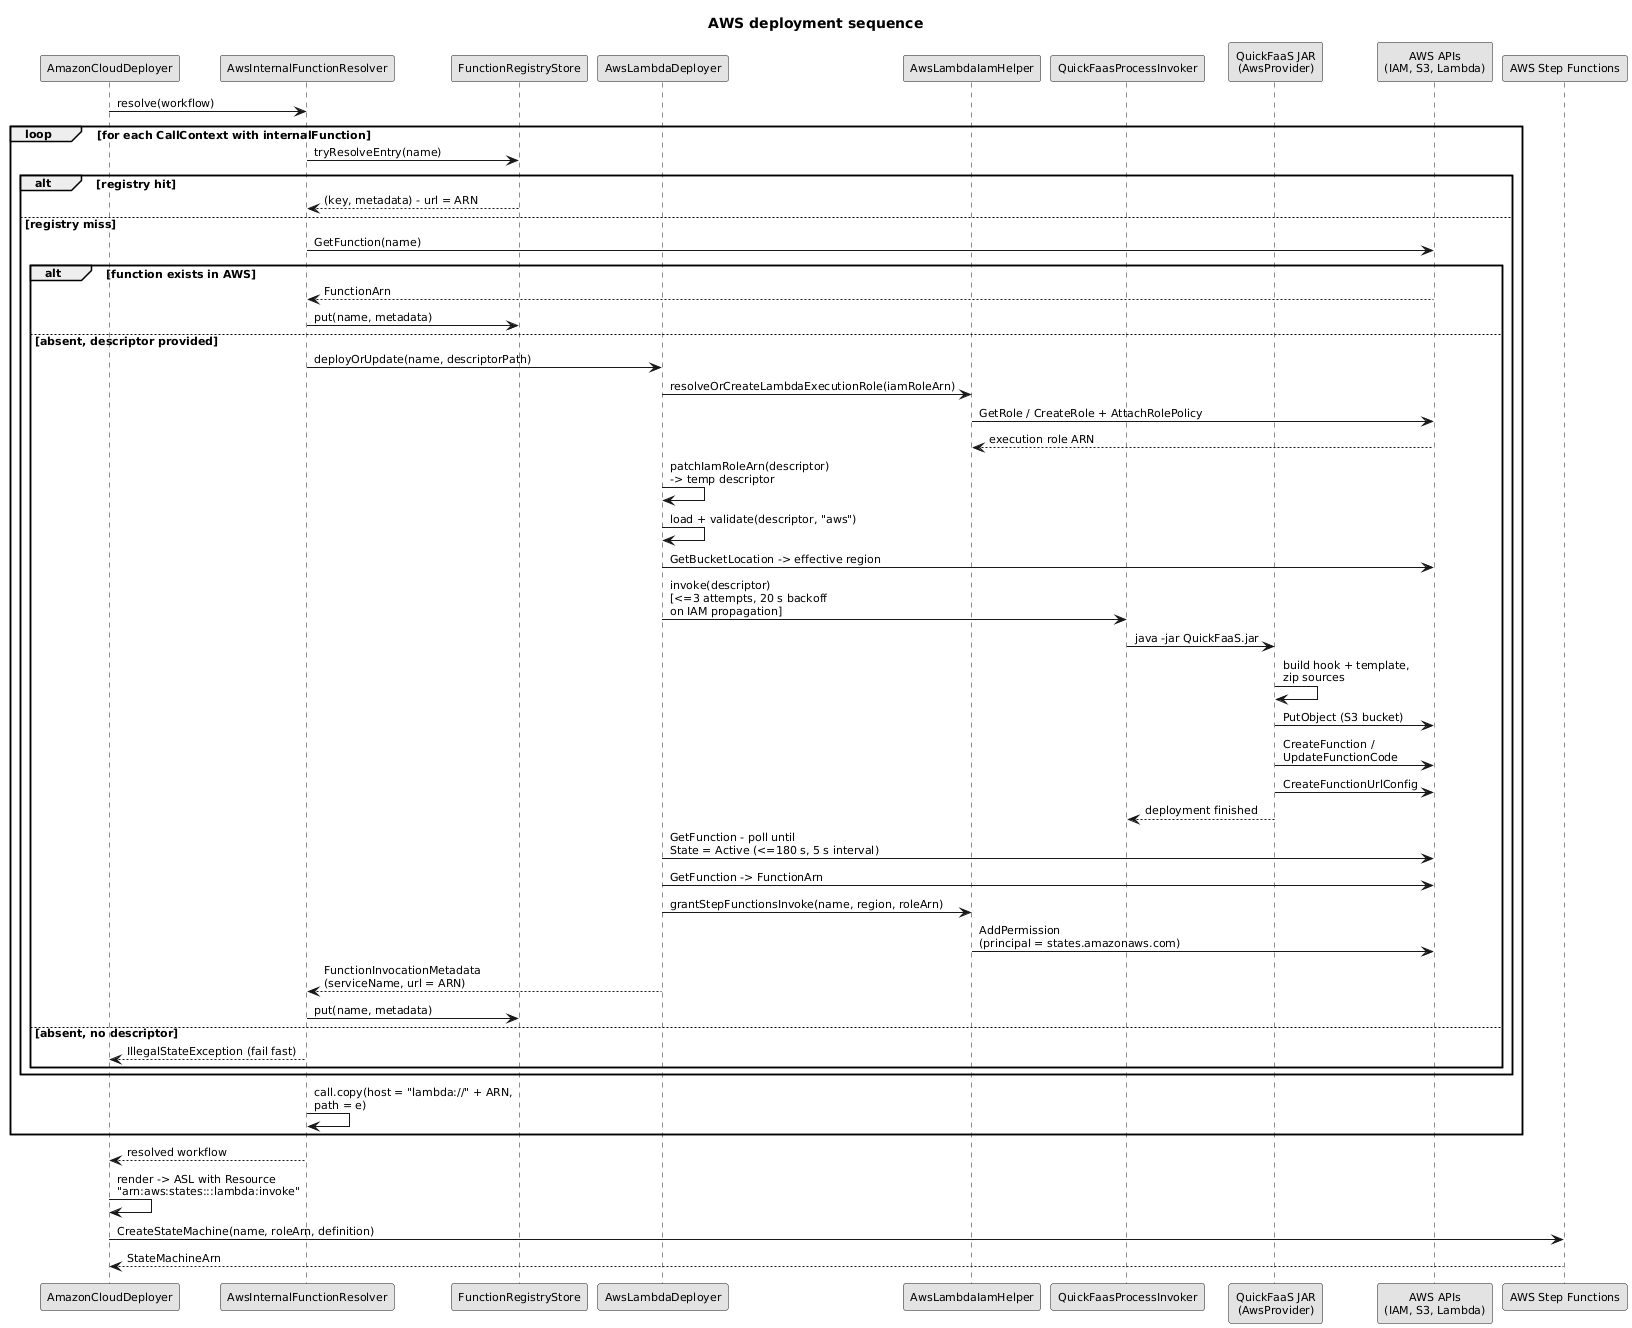
\includegraphics[width=\textwidth]{images/implementation/aws-deploy-sequence.png}
  \caption{Deployment sequence on AWS for the worst-case path (function absent from
  both the registry and the provider).}
  \label{fig:aws-deploy-sequence}
\end{figure}

AWS support is realised in two layers that meet at the subprocess boundary: the AWS provider added
\emph{inside} QuickFaaS, which performs the actual Lambda deployment, and the
\texttt{AwsLambdaDeployer} added \emph{inside} OmniFlow, which prepares the environment,
drives QuickFaaS, and produces the invocation metadata the registry stores.

\subsection{The QuickFaaS AWS Provider}
\label{subsec:quickfaas-aws-provider}

The AWS provider extends QuickFaaS's existing abstractions (\texttt{CloudProvider},
\texttt{CloudFunction}, \texttt{CloudRequests}) so that a cloud-agnostic function can be packaged
and deployed to AWS Lambda through the same ZIP strategy used for GCP and Azure. Its core is
\texttt{AwsLambdaFunction.deployZip}, which: uploads the packaged archive to the S3 bucket named in
the descriptor; checks whether the function already exists (\texttt{GetFunction}); and then either
creates it (\texttt{CreateFunction}, with the code referenced as an S3 object) or updates its code
(\texttt{UpdateFunctionCode}), in both cases blocking on the AWS SDK waiter until the function is
active. The handler is fixed to the provider-agnostic entry point \texttt{AwsHttpTemplate}, which
adapts the Lambda request to the developer's hook, and the supported runtimes are \texttt{java11}
and \texttt{java17}. Because \texttt{GetBucketLocation} must be issued against the global endpoint,
the provider resolves the bucket's region from \texttt{us-east-1} and then pins the Lambda client
to that same region, ensuring the function and its code bucket are co-located. Finally, the
provider creates (or reuses) a Lambda \emph{Function URL} with \texttt{AuthType = AWS\_IAM}. This
Function URL is QuickFaaS's own notion of an invocation endpoint; as explained below, the OmniFlow
integration does not use it, preferring the function ARN.

\subsection{The OmniFlow-Side Deployer}
\label{subsec:omniflow-aws-deployer}

\texttt{AwsLambdaDeployer} is the AWS implementation of the \texttt{InternalFunctionDeployer}
strategy. It performs the work that has no GCP equivalent and that must happen \emph{around} the
QuickFaaS subprocess. From the raw descriptor it resolves or creates the Lambda execution IAM role:
if \texttt{iamRoleArn} is blank or a placeholder, it creates a managed
\texttt{OmniFlowLambdaExecutionRole} (attaching \texttt{AWSLambdaBasicExecutionRole}); if a real ARN
is supplied, it verifies and, if necessary, repairs the role's trust policy so that
\texttt{lambda.amazonaws.com} can assume it. The resolved ARN is patched into a temporary copy of
the descriptor, the effective region is taken from the S3 bucket's location, and QuickFaaS is
invoked as a subprocess --- retried up to three times with a 20-second back-off to absorb IAM
eventual consistency. After the subprocess returns, the deployer polls \texttt{GetFunction} until
the function reports the \texttt{Active} state (bounded by a 180-second timeout), retrieves the ARN,
and grants the Step Functions service principal permission to invoke the function.

A deliberate design choice is visible here: although the QuickFaaS provider produces a Function URL,
the OmniFlow deployer discards it and stores the \emph{ARN} in the registry, because internal calls
are rendered with the native \texttt{lambda:invoke} integration (Section~\ref{sec:runtime-invocation})
rather than as HTTP calls to a Function URL. Listing~\ref{lst:aws-descriptor} shows a minimal AWS
deployment descriptor: it differs from the GCP descriptor of
Listing~\ref{lst:quickfaas_json_config} mainly in \texttt{cloudProvider}, the S3 \texttt{bucket},
the Lambda \texttt{runtime}, and the \texttt{iamRoleArn} field (which may be left as a placeholder to
request automatic role creation).

\begin{lstlisting}[language=json,caption={Minimal AWS deployment descriptor for an internal function.},label={lst:aws-descriptor}]
{
  "cloudProvider": "aws",
  "project": "123456789012",
  "iamRoleArn": "<auto>",
  "function": {
    "name": "hello-lambda-fn",
    "location": "eu-west-1",
    "bucket": "run-sources-tfm2526-eu-west-1",
    "runtime": "java17",
    "trigger": { "type": "http" }
  },
  "functionFile": "./MyFunctionClass.java"
}
\end{lstlisting}

\section{Runtime Invocation}
\label{sec:runtime-invocation}
Figure~\ref{fig:aws-runtime-invocation} shows how an internal function is invoked at runtime, once the workflow is deployed. Unlike external calls — which are rendered as \texttt{apigateway:invoke} HTTP tasks — internal calls use the native \texttt{arn:aws:states:::lambda:invoke} integration, with the ARN fixed at deployment time. Step Functions invokes the Lambda directly with the step's payload; the QuickFaaS template entry point adapts the request and delegates to the developer's hook function, and the response is returned under \texttt{\$.Payload}, from which a \texttt{ResultSelector} extracts the value into the step's result variable. Using the native integration rather than an HTTP endpoint avoids per-call request signing and keeps the invocation within the AWS control plane; this choice is confirmed by the renderer, whose emitted resource for internal calls is \texttt{lambda:invoke} (\texttt{AmazonConstantsUtils}).

\begin{figure}[htbp]
  \centering
  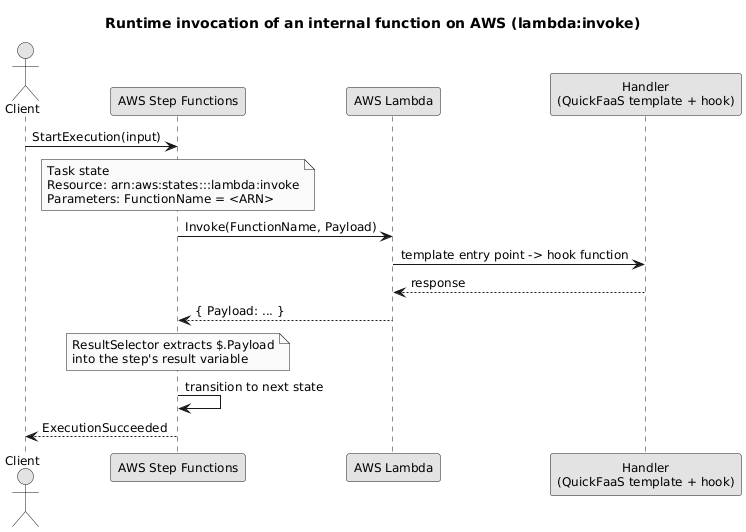
\includegraphics[width=0.8\textwidth]{images/implementation/aws-runtime-invocation.png}
  \caption{Runtime invocation of an internal function on AWS via the native
  \texttt{lambda:invoke} integration.}
  \label{fig:aws-runtime-invocation}
\end{figure}

The distinction between the two forms is made entirely by the renderer,
\texttt{AmazonCallRenderer}, from the \texttt{host} value injected during resolution. If the host
carries the \texttt{lambda://} prefix (the marker written by \texttt{Aws\allowbreak Internal\allowbreak Function\allowbreak Resolver}),
the renderer emits a \texttt{Task} whose \texttt{Resource} is
\texttt{arn:aws:states:::lambda:invoke} and whose \texttt{Parameters} carry the
\texttt{FunctionName} taken from the resolved ARN; any query terms are forwarded under a
\texttt{Payload.queryStringParameters} object. Otherwise it emits the original
\texttt{apigateway:invoke} task with \texttt{ApiEndpoint}, \texttt{Method} and \texttt{Path}. For
the Lambda form the result is extracted with a \texttt{ResultSelector} that reads
\texttt{\$.Payload} into the step's result variable, and the value is scoped under a
\texttt{ResultPath} named after the step so that later steps can reference it. Listing
\ref{lst:rendered-lambda} shows the state a \texttt{call} to \texttt{internalFunction("fraud-check")}
renders to.

\begin{lstlisting}[language=json,caption={Step Functions state rendered for an internal Lambda call.},label={lst:rendered-lambda}]
"fraud-check": {
  "Type": "Task",
  "Resource": "arn:aws:states:::lambda:invoke",
  "InputPath": "$",
  "Parameters": {
    "FunctionName": "arn:aws:lambda:eu-west-1:123456789012:function:fraud-check"
  },
  "ResultSelector": { "fraudResult.$": "$.Payload" },
  "ResultPath": "$.fraud-check",
  "Next": "external-risk-api"
}
\end{lstlisting}

Keeping the internal form as a variant of the existing \texttt{call} renderer --- rather than a new
state type --- means the control-flow, result-passing and error-handling machinery that OmniFlow
already emits for external calls applies unchanged to internal ones; only the \texttt{Resource} and
the parameter shape differ.
%\lipsum[1-100]
% \lipsum[1-100]
% \lipsum[1-100]
% \lipsum[1-700]

